\documentclass[aspectratio=169,12pt]{beamer}

% Theme and colors
\usetheme{Madrid}
\usecolortheme{whale}
\setbeamertemplate{navigation symbols}{}
\setbeamertemplate{footline}[frame number]

% Packages
\usepackage{graphicx}
\usepackage{tikz}
\usetikzlibrary{shapes,arrows,positioning,calc,matrix}
\usepackage{booktabs}
\usepackage{array}
\usepackage{xcolor}
\usepackage{hyperref}

% Custom colors
\definecolor{codegreen}{rgb}{0,0.6,0}
\definecolor{codepurple}{rgb}{0.58,0,0.82}
\definecolor{darkblue}{rgb}{0,0,0.7}

% Title information
\title[JPEG Baseline Coding]{JPEG Baseline Coding}
\subtitle{How Your Photos Get Compressed}
\author[Mahesh C]{\textbf{Mahesh C}\\FISAT}
\institute{Federal Institute of Science and Technology (FISAT)\\Multimedia Technology Class}
\date{\today}

\begin{document}

% Title slide
\begin{frame}
    \titlepage
\end{frame}

% Outline
\begin{frame}{Outline}
    \tableofcontents
\end{frame}

%==============================================================================
\section{Why Do We Need JPEG?}
%==============================================================================

\begin{frame}{A Simple Question}
    \begin{center}
        \Huge{How big is a single photo from your phone?}
    \end{center}
    
    \vspace{1cm}
    \pause
    \begin{columns}
        \begin{column}{0.5\textwidth}
            \textbf{Without compression:}
            \begin{itemize}
                \item 12 MP camera = 12 million pixels
                \item Each pixel = 3 colors (RGB)
                \item Each color = 1 byte
                \item Total = 36 MB per photo!
            \end{itemize}
        \end{column}
        \begin{column}{0.5\textwidth}
            \textbf{With JPEG:}
            \begin{itemize}
                \item Same 12 MP photo
                \item Only 2-4 MB
                \item 90\% smaller!
                \item Still looks great
            \end{itemize}
        \end{column}
    \end{columns}
\end{frame}

\begin{frame}{Real Life Impact}
    \begin{alertblock}{Think About This}
        Your phone has 128 GB storage. Without JPEG:
        \begin{itemize}
            \item You could store only \textbf{3,500 photos}
            \item With JPEG: \textbf{35,000+ photos}!
        \end{itemize}
    \end{alertblock}
    
    \vspace{0.5cm}
    \textbf{JPEG saves the day everywhere:}
    \begin{itemize}
        \item \textbf{WhatsApp:} Sends photos in seconds, not minutes
        \item \textbf{Instagram:} Millions of photos uploaded daily
        \item \textbf{Websites:} Pages load fast with JPEG images
        \item \textbf{Email:} Attach photos without hitting size limits
    \end{itemize}
\end{frame}

\begin{frame}{What is JPEG?}
    \begin{block}{JPEG = Joint Photographic Experts Group}
        A committee that created the standard in 1992. Still the most popular image format today!
    \end{block}
    
    \vspace{0.5cm}
    \textbf{Key Facts:}
    \begin{itemize}
        \item \textbf{Lossy compression} --- throws away some data you won't notice
        \item \textbf{Best for photos} --- not good for text, logos, or screenshots
        \item \textbf{Adjustable quality} --- you choose size vs quality tradeoff
        \item \textbf{Universal} --- works on every device, browser, app
    \end{itemize}
    
    \vspace{0.3cm}
    \begin{center}
        \textit{``Good enough'' quality at a fraction of the size}
    \end{center}
\end{frame}

%==============================================================================
\section{The Big Picture: JPEG Pipeline}
%==============================================================================

\begin{frame}{JPEG Compression: The Journey of a Photo}
    \begin{center}
        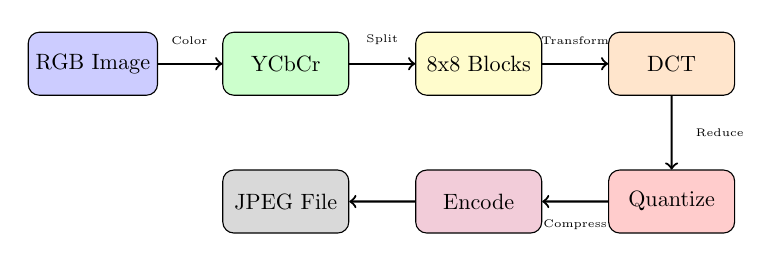
\begin{tikzpicture}[scale=0.7, every node/.style={scale=0.8}]
            % Step boxes
            \node[draw, fill=blue!20, minimum width=2cm, minimum height=1cm, rounded corners] (rgb) at (0,0) {RGB Image};
            \node[draw, fill=green!20, minimum width=2cm, minimum height=1cm, rounded corners] (ycbcr) at (3.5,0) {YCbCr};
            \node[draw, fill=yellow!20, minimum width=2cm, minimum height=1cm, rounded corners] (blocks) at (7,0) {8x8 Blocks};
            \node[draw, fill=orange!20, minimum width=2cm, minimum height=1cm, rounded corners] (dct) at (10.5,0) {DCT};
            \node[draw, fill=red!20, minimum width=2cm, minimum height=1cm, rounded corners] (quant) at (10.5,-2.5) {Quantize};
            \node[draw, fill=purple!20, minimum width=2cm, minimum height=1cm, rounded corners] (encode) at (7,-2.5) {Encode};
            \node[draw, fill=gray!30, minimum width=2cm, minimum height=1cm, rounded corners] (jpeg) at (3.5,-2.5) {JPEG File};
            
            % Arrows
            \draw[->,thick] (rgb) -- (ycbcr);
            \draw[->,thick] (ycbcr) -- (blocks);
            \draw[->,thick] (blocks) -- (dct);
            \draw[->,thick] (dct) -- (quant);
            \draw[->,thick] (quant) -- (encode);
            \draw[->,thick] (encode) -- (jpeg);
            
            % Labels
            \node[above] at (1.75,0.2) {\tiny Color};
            \node[above] at (5.25,0.2) {\tiny Split};
            \node[above] at (8.75,0.2) {\tiny Transform};
            \node[right] at (10.8,-1.25) {\tiny Reduce};
            \node[below] at (8.75,-2.7) {\tiny Compress};
        \end{tikzpicture}
    \end{center}
    
    \vspace{0.5cm}
    \textbf{Six simple steps:}
    \begin{enumerate}
        \item Change colors from RGB to YCbCr
        \item Split image into small 8x8 pixel blocks
        \item Transform each block (DCT magic)
        \item Throw away details you won't see (Quantization)
        \item Compress the numbers (Huffman coding)
        \item Save as JPEG file
    \end{enumerate}
\end{frame}

\begin{frame}{Think of it Like Packing for a Trip}
    \begin{columns}
        \begin{column}{0.5\textwidth}
            \textbf{Packing a suitcase:}
            \begin{enumerate}
                \item Sort clothes by type
                \item Fold into small bundles
                \item Remove wrinkles (organize)
                \item Leave behind things you won't need
                \item Compress everything tight
                \item Zip up the suitcase
            \end{enumerate}
        \end{column}
        \begin{column}{0.5\textwidth}
            \textbf{JPEG compression:}
            \begin{enumerate}
                \item Sort colors (RGB $\rightarrow$ YCbCr)
                \item Split into 8x8 blocks
                \item Organize data (DCT)
                \item Remove invisible details
                \item Compress numbers (Huffman)
                \item Save as file
            \end{enumerate}
        \end{column}
    \end{columns}
    
    \vspace{0.5cm}
    \begin{block}{The Goal}
        Keep what matters, remove what doesn't, pack it efficiently!
    \end{block}
\end{frame}

%==============================================================================
\section{Step 1: Color Space Conversion}
%==============================================================================

\begin{frame}{Why Change Colors? RGB vs YCbCr}
    \begin{columns}
        \begin{column}{0.5\textwidth}
            \textbf{RGB (What cameras capture):}
            \begin{itemize}
                \item Red, Green, Blue
                \item Each pixel = 3 values
                \item All three equally important
                \item Computer-friendly
            \end{itemize}
            
            \vspace{0.3cm}
            \textbf{Problem:}
            
            Can't compress any channel more than others --- all seem equally important!
        \end{column}
        \begin{column}{0.5\textwidth}
            \textbf{YCbCr (What JPEG uses):}
            \begin{itemize}
                \item Y = Brightness (Luminance)
                \item Cb = Blue-ish color
                \item Cr = Red-ish color
            \end{itemize}
            
            \vspace{0.3cm}
            \textbf{Advantage:}
            
            Human eyes care more about brightness than color details!
        \end{column}
    \end{columns}
\end{frame}

\begin{frame}{The Human Eye Trick}
    \begin{alertblock}{Scientific Fact}
        Your eyes have 120 million cells for brightness but only 6 million for color!
    \end{alertblock}
    
    \vspace{0.5cm}
    \textbf{What this means for JPEG:}
    \begin{itemize}
        \item Keep full detail for brightness (Y)
        \item Reduce detail for colors (Cb, Cr) --- you won't notice!
        \item This alone saves 50\% of data
    \end{itemize}
    
    \vspace{0.5cm}
    \begin{block}{Real Example}
        A 1000x1000 pixel image:
        \begin{itemize}
            \item Y: Keep all 1,000,000 values
            \item Cb: Keep only 250,000 values (1/4)
            \item Cr: Keep only 250,000 values (1/4)
        \end{itemize}
        Result: 1.5 million values instead of 3 million!
    \end{block}
\end{frame}

\begin{frame}{Chroma Subsampling: The Secret Sauce}
    \begin{center}
        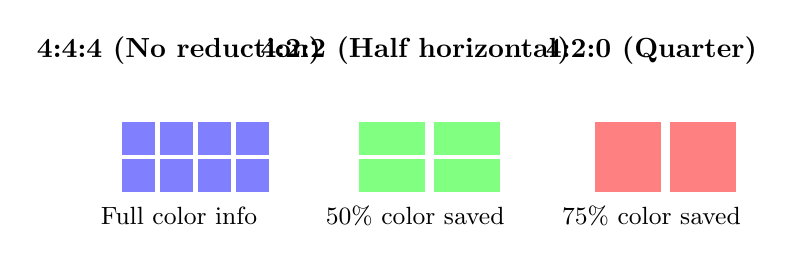
\begin{tikzpicture}[scale=0.6]
            % 4:4:4
            \node at (0,3) {\textbf{4:4:4 (No reduction)}};
            \foreach \x in {0,1,2,3} {
                \foreach \y in {0,1} {
                    \fill[blue!50] (\x*0.8-1.2, \y*0.8) rectangle (\x*0.8-0.5, \y*0.8+0.7);
                }
            }
            \node at (0,-0.5) {\small Full color info};
            
            % 4:2:2
            \node at (5,3) {\textbf{4:2:2 (Half horizontal)}};
            \foreach \x in {0,1} {
                \foreach \y in {0,1} {
                    \fill[green!50] (\x*1.6+3.8, \y*0.8) rectangle (\x*1.6+5.2, \y*0.8+0.7);
                }
            }
            \node at (5,-0.5) {\small 50\% color saved};
            
            % 4:2:0
            \node at (10,3) {\textbf{4:2:0 (Quarter)}};
            \foreach \x in {0,1} {
                \foreach \y in {0} {
                    \fill[red!50] (\x*1.6+8.8, \y*1.6) rectangle (\x*1.6+10.2, \y*1.6+1.5);
                }
            }
            \node at (10,-0.5) {\small 75\% color saved};
        \end{tikzpicture}
    \end{center}
    
    \vspace{0.5cm}
    \textbf{Most JPEGs use 4:2:0:}
    \begin{itemize}
        \item Every 2x2 block of pixels shares one color value
        \item You can't tell the difference in photos!
        \item Huge space savings with no visible quality loss
    \end{itemize}
\end{frame}

%==============================================================================
\section{Step 2: Block Splitting}
%==============================================================================

\begin{frame}{Why 8x8 Blocks?}
    \begin{columns}
        \begin{column}{0.5\textwidth}
            \textbf{The Idea:}
            
            Instead of processing the whole image at once, split it into tiny 8x8 pixel squares.
            
            \vspace{0.5cm}
            \textbf{Why 8x8?}
            \begin{itemize}
                \item Small enough to be similar inside
                \item Big enough to find patterns
                \item Perfect for the math that comes next
                \item Good balance of speed and quality
            \end{itemize}
        \end{column}
        \begin{column}{0.5\textwidth}
            \begin{center}
                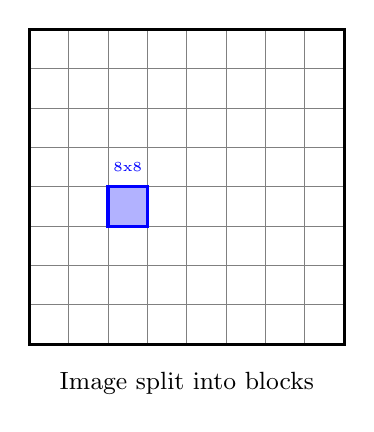
\begin{tikzpicture}[scale=0.5]
                    % Image grid
                    \draw[step=1, gray, thin] (0,0) grid (8,8);
                    \draw[very thick] (0,0) rectangle (8,8);
                    
                    % Highlight one block
                    \fill[blue!30] (2,3) rectangle (3,4);
                    \draw[blue, very thick] (2,3) rectangle (3,4);
                    
                    % Labels
                    \node at (4,-1) {\small Image split into blocks};
                    \node[blue] at (2.5,4.5) {\tiny 8x8};
                \end{tikzpicture}
            \end{center}
            
            \vspace{0.3cm}
            \textbf{Example:}
            
            A 1920x1080 image = 32,400 blocks
            
            Each processed independently!
        \end{column}
    \end{columns}
\end{frame}

\begin{frame}{What's Inside a Block?}
    \begin{columns}
        \begin{column}{0.5\textwidth}
            \textbf{A typical 8x8 block:}
            \begin{center}
                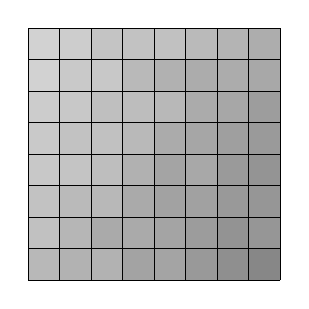
\begin{tikzpicture}[scale=0.4]
                    \foreach \x in {0,...,7} {
                        \foreach \y in {0,...,7} {
                            \pgfmathsetmacro{\shade}{50 + 5*\x - 3*\y + random(0,10)}
                            \fill[gray!\shade] (\x,\y) rectangle (\x+1,\y+1);
                        }
                    }
                    \draw[step=1, black, thin] (0,0) grid (8,8);
                \end{tikzpicture}
            \end{center}
            
            64 pixels, each with a brightness value (0-255)
        \end{column}
        \begin{column}{0.5\textwidth}
            \textbf{Key observation:}
            
            Neighboring pixels are usually similar!
            
            \vspace{0.3cm}
            \begin{itemize}
                \item Sky: all similar blue
                \item Skin: smooth gradients
                \item Grass: similar greens
            \end{itemize}
            
            \vspace{0.3cm}
            \textbf{This similarity = redundancy}
            
            Redundancy = opportunity to compress!
        \end{column}
    \end{columns}

\end{frame}

%==============================================================================
\section{Step 3: DCT --- The Magic Transform}
%==============================================================================

\begin{frame}{DCT: Don't Worry About the Math!}
    \begin{block}{What DCT Does (Simple Version)}
        Converts pixel values into ``frequency'' information.
        
        Think of it as finding patterns in the block.
    \end{block}
    
    \vspace{0.5cm}
    \textbf{Analogy: Music Equalizer}
    \begin{itemize}
        \item Music has bass (low frequency) and treble (high frequency)
        \item An equalizer shows how much of each
        \item DCT does the same for images!
    \end{itemize}
    
    \vspace{0.3cm}
    \begin{columns}
        \begin{column}{0.5\textwidth}
            \textbf{Low frequency =}
            \begin{itemize}
                \item Smooth areas
                \item Gradual changes
                \item The ``big picture''
            \end{itemize}
        \end{column}
        \begin{column}{0.5\textwidth}
            \textbf{High frequency =}
            \begin{itemize}
                \item Sharp edges
                \item Fine details
                \item Texture and noise
            \end{itemize}
        \end{column}
    \end{columns}
\end{frame}

\begin{frame}{Before and After DCT}
    \begin{columns}
        \begin{column}{0.5\textwidth}
            \textbf{Before DCT:}
            
            64 pixel values scattered all over
            
            \begin{center}
                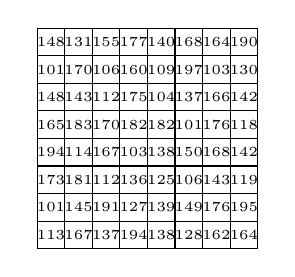
\begin{tikzpicture}[scale=0.35]
                    \foreach \x in {0,...,7} {
                        \foreach \y in {0,...,7} {
                            \pgfmathsetmacro{\val}{int(100 + random(0,100))}
                            \node[font=\tiny] at (\x+0.5, \y+0.5) {\val};
                        }
                    }
                    \draw[step=1] (0,0) grid (8,8);
                \end{tikzpicture}
            \end{center}
            
            All values seem important
        \end{column}
        \begin{column}{0.5\textwidth}
            \textbf{After DCT:}
            
            Energy concentrated in corner!
            
            \begin{center}
                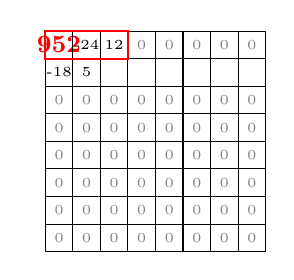
\begin{tikzpicture}[scale=0.35]
                    % Big value in corner
                    \node[font=\small, red] at (0.5, 7.5) {\textbf{952}};
                    % Smaller values nearby
                    \node[font=\tiny] at (1.5, 7.5) {-24};
                    \node[font=\tiny] at (2.5, 7.5) {12};
                    \node[font=\tiny] at (0.5, 6.5) {-18};
                    \node[font=\tiny] at (1.5, 6.5) {5};
                    % Rest are small or zero
                    \foreach \x in {3,...,7} {
                        \node[font=\tiny, gray] at (\x+0.5, 7.5) {0};
                    }
                    \foreach \y in {0,...,5} {
                        \foreach \x in {0,...,7} {
                            \node[font=\tiny, gray] at (\x+0.5, \y+0.5) {0};
                        }
                    }
                    \draw[step=1] (0,0) grid (8,8);
                    \draw[red, thick] (0,7) rectangle (3,8);
                \end{tikzpicture}
            \end{center}
            
            Most values are zero or tiny!
        \end{column}
    \end{columns}
    
    \vspace{0.3cm}
    \begin{alertblock}{The Magic}
        DCT doesn't compress anything yet --- it just reorganizes data so compression becomes easy!
    \end{alertblock}
\end{frame}

\begin{frame}{The DCT Coefficient Map}
    \begin{center}
        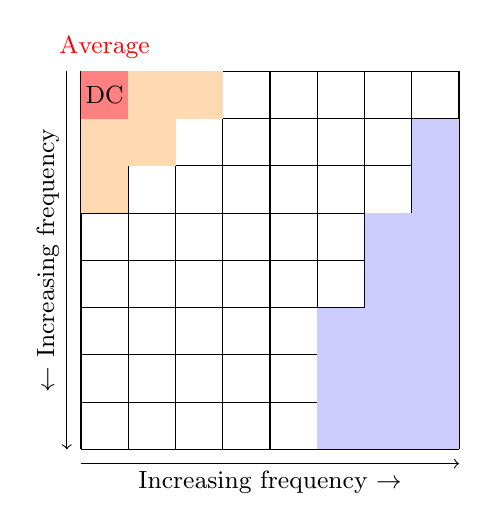
\begin{tikzpicture}[scale=0.6]
            % Draw 8x8 grid
            \draw[step=1] (0,0) grid (8,8);
            
            % DC coefficient
            \fill[red!50] (0,7) rectangle (1,8);
            \node at (0.5,7.5) {\small DC};
            
            % Low frequency area
            \fill[orange!30] (1,7) rectangle (3,8);
            \fill[orange!30] (0,5) rectangle (1,7);
            \fill[orange!30] (1,6) rectangle (2,7);
            
            % High frequency area
            \fill[blue!20] (5,0) rectangle (8,3);
            \fill[blue!20] (6,3) rectangle (8,5);
            \fill[blue!20] (7,5) rectangle (8,7);
            
            % Labels
            \node[red] at (0.5,8.5) {\small Average};
            \node at (4,-0.7) {\small Increasing frequency $\rightarrow$};
            \draw[->] (0,-0.3) -- (8,-0.3);
            
            % Side label
            \node[rotate=90] at (-0.7,4) {\small $\leftarrow$ Increasing frequency};
            \draw[->] (-0.3,8) -- (-0.3,0);
        \end{tikzpicture}
    \end{center}
    
    \vspace{0.3cm}
    \begin{itemize}
        \item \textcolor{red}{\textbf{Top-left (DC):}} Average brightness of the block
        \item \textcolor{orange}{\textbf{Near top-left:}} Low frequency = smooth patterns (important!)
        \item \textcolor{blue}{\textbf{Bottom-right:}} High frequency = fine details (often ignorable)
    \end{itemize}
\end{frame}

%==============================================================================
\section{Step 4: Quantization --- Where Quality is Lost}
%==============================================================================

\begin{frame}{Quantization: The Lossy Step}
    \begin{alertblock}{This is where JPEG becomes ``lossy''}
        Quantization throws away information you (hopefully) won't miss!
    \end{alertblock}
    
    \vspace{0.5cm}
    \textbf{Simple Analogy: Rounding Money}
    \begin{itemize}
        \item You have \$47.83
        \item Round to nearest \$10 $\rightarrow$ \$50
        \item You lost \$2.17 of precision
        \item But for rough estimates, \$50 is ``good enough''
    \end{itemize}
    
    \vspace{0.3cm}
    \textbf{JPEG does the same:}
    \begin{itemize}
        \item DCT gives precise values like 47.83
        \item Quantization rounds them: 47.83 $\rightarrow$ 5
        \item Less precise, but much smaller numbers!
    \end{itemize}
\end{frame}

\begin{frame}{The Quantization Table}
    \begin{columns}
        \begin{column}{0.5\textwidth}
            \textbf{Divide each DCT value by a number:}
            
            \begin{center}
                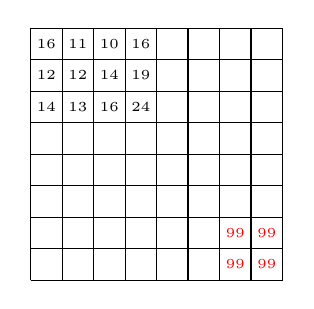
\begin{tikzpicture}[scale=0.4]
                    % Quantization table (simplified)
                    \node[font=\tiny] at (0.5,7.5) {16};
                    \node[font=\tiny] at (1.5,7.5) {11};
                    \node[font=\tiny] at (2.5,7.5) {10};
                    \node[font=\tiny] at (3.5,7.5) {16};
                    \node[font=\tiny] at (0.5,6.5) {12};
                    \node[font=\tiny] at (1.5,6.5) {12};
                    \node[font=\tiny] at (2.5,6.5) {14};
                    \node[font=\tiny] at (3.5,6.5) {19};
                    \node[font=\tiny] at (0.5,5.5) {14};
                    \node[font=\tiny] at (1.5,5.5) {13};
                    \node[font=\tiny] at (2.5,5.5) {16};
                    \node[font=\tiny] at (3.5,5.5) {24};
                    % High frequency = big divisors
                    \node[font=\tiny, red] at (6.5,1.5) {99};
                    \node[font=\tiny, red] at (7.5,1.5) {99};
                    \node[font=\tiny, red] at (6.5,0.5) {99};
                    \node[font=\tiny, red] at (7.5,0.5) {99};
                    \draw[step=1] (0,0) grid (8,8);
                \end{tikzpicture}
            \end{center}
            
            \small Small divisors (top-left) = keep detail
            
            \small \textcolor{red}{Big divisors (bottom-right) = lose detail}
        \end{column}
        \begin{column}{0.5\textwidth}
            \textbf{Example:}
            
            DCT value = 95
            
            Quantization divisor = 16
            
            Result = round(95/16) = \textbf{6}
            
            \vspace{0.5cm}
            \textbf{High frequency example:}
            
            DCT value = 12
            
            Quantization divisor = 99
            
            Result = round(12/99) = \textbf{0}
            
            \vspace{0.3cm}
            \textit{Small details become zero!}
        \end{column}
    \end{columns}
\end{frame}

\begin{frame}{Quality Settings Explained}
    \begin{center}
        \Large{What does ``JPEG Quality 80\%'' mean?}
    \end{center}
    
    \vspace{0.5cm}
    \begin{columns}
        \begin{column}{0.33\textwidth}
            \textbf{Quality 100\%}
            \begin{itemize}
                \item Small divisors
                \item Keep most detail
                \item Larger file
                \item Best quality
            \end{itemize}
        \end{column}
        \begin{column}{0.33\textwidth}
            \textbf{Quality 75\%}
            \begin{itemize}
                \item Medium divisors
                \item Good balance
                \item Reasonable size
                \item \textit{Most common}
            \end{itemize}
        \end{column}
        \begin{column}{0.33\textwidth}
            \textbf{Quality 20\%}
            \begin{itemize}
                \item Large divisors
                \item Lose lots of detail
                \item Tiny file
                \item Visible artifacts
            \end{itemize}
        \end{column}
    \end{columns}
    
    \vspace{0.5cm}
    \begin{block}{Rule of Thumb}
        Quality 70-85\% is usually the sweet spot --- good quality, reasonable size.
    \end{block}
\end{frame}

\begin{frame}{What Happens at Low Quality?}
    \textbf{JPEG Artifacts --- Signs of Over-Compression:}
    
    \vspace{0.5cm}
    \begin{columns}
        \begin{column}{0.5\textwidth}
            \textbf{1. Blocking}
            \begin{itemize}
                \item 8x8 block boundaries become visible
                \item Smooth areas look ``blocky''
                \item Like a mosaic effect
            \end{itemize}
            
            \vspace{0.3cm}
            \textbf{2. Ringing}
            \begin{itemize}
                \item Halos around sharp edges
                \item ``Ghosting'' near text
                \item Wavy patterns
            \end{itemize}
        \end{column}
        \begin{column}{0.5\textwidth}
            \textbf{3. Color Bleeding}
            \begin{itemize}
                \item Colors smear into each other
                \item Red bleeds into white
                \item Especially around edges
            \end{itemize}
            
            \vspace{0.3cm}
            \textbf{4. Mosquito Noise}
            \begin{itemize}
                \item Fuzzy dots around edges
                \item Looks like tiny insects
                \item Common in video too
            \end{itemize}
        \end{column}
    \end{columns}
\end{frame}

%==============================================================================
\section{Step 5: Entropy Coding}
%==============================================================================

\begin{frame}{After Quantization: Lots of Zeros!}
    \textbf{A typical quantized block:}
    
    \begin{center}
        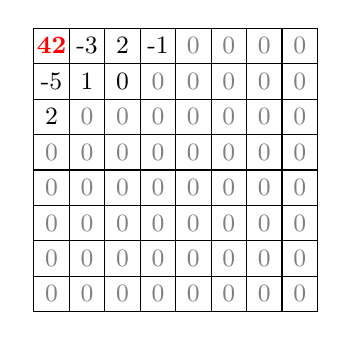
\begin{tikzpicture}[scale=0.45]
            % Values after quantization
            \node[font=\small, red] at (0.5,7.5) {\textbf{42}};
            \node[font=\small] at (1.5,7.5) {-3};
            \node[font=\small] at (2.5,7.5) {2};
            \node[font=\small] at (3.5,7.5) {-1};
            \node[font=\small] at (0.5,6.5) {-5};
            \node[font=\small] at (1.5,6.5) {1};
            \node[font=\small] at (2.5,6.5) {0};
            \node[font=\small, gray] at (3.5,6.5) {0};
            \node[font=\small] at (0.5,5.5) {2};
            \node[font=\small, gray] at (1.5,5.5) {0};
            \node[font=\small, gray] at (2.5,5.5) {0};
            \node[font=\small, gray] at (3.5,5.5) {0};
            % Rest are zeros
            \foreach \x in {4,...,7} {
                \foreach \y in {5,...,7} {
                    \node[font=\small, gray] at (\x+0.5,\y+0.5) {0};
                }
            }
            \foreach \y in {0,...,4} {
                \foreach \x in {0,...,7} {
                    \node[font=\small, gray] at (\x+0.5,\y+0.5) {0};
                }
            }
            \draw[step=1] (0,0) grid (8,8);
        \end{tikzpicture}
    \end{center}
    
    \vspace{0.3cm}
    \textbf{Notice:} Most values are 0! Only a few non-zero values in the top-left.
    
    \textbf{Opportunity:} Instead of storing 64 numbers, just store the non-zero ones!
\end{frame}

\begin{frame}{Zigzag Scan: Reading the Block}
    \begin{columns}
        \begin{column}{0.5\textwidth}
            \textbf{Read in zigzag order:}
            
            \begin{center}
                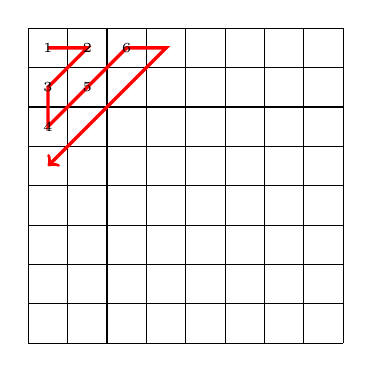
\begin{tikzpicture}[scale=0.5]
                    \draw[step=1] (0,0) grid (8,8);
                    % Zigzag path
                    \draw[red, very thick, ->] 
                        (0.5,7.5) -- (1.5,7.5) -- (0.5,6.5) -- (0.5,5.5) -- 
                        (1.5,6.5) -- (2.5,7.5) -- (3.5,7.5) -- (2.5,6.5) --
                        (1.5,5.5) -- (0.5,4.5);
                    % Numbers
                    \node[font=\tiny] at (0.5,7.5) {1};
                    \node[font=\tiny] at (1.5,7.5) {2};
                    \node[font=\tiny] at (0.5,6.5) {3};
                    \node[font=\tiny] at (0.5,5.5) {4};
                    \node[font=\tiny] at (1.5,6.5) {5};
                    \node[font=\tiny] at (2.5,7.5) {6};
                \end{tikzpicture}
            \end{center}
        \end{column}
        \begin{column}{0.5\textwidth}
            \textbf{Why zigzag?}
            \begin{itemize}
                \item Groups low frequencies first
                \item High frequencies (zeros) come last
                \item Long runs of zeros at the end
                \item Easy to compress!
            \end{itemize}
            
            \vspace{0.3cm}
            \textbf{Result:}
            
            42, -3, -5, 2, 1, 2, -1, 0, 0, 0, 0, 0, ... (lots of zeros)
        \end{column}
    \end{columns}

\end{frame}

\begin{frame}{Run-Length and Huffman Coding}
    \textbf{Two tricks to compress the zigzag sequence:}
    
    \vspace{0.5cm}
    \begin{columns}
        \begin{column}{0.5\textwidth}
            \textbf{1. Run-Length Encoding}
            
            Instead of: 5, 0, 0, 0, 0, 3
            
            Write: 5, (4 zeros), 3
            
            Or even shorter: (0,5), (4,3)
            
            \vspace{0.3cm}
            \textit{``Skip 0 zeros, value is 5''}
            
            \textit{``Skip 4 zeros, value is 3''}
        \end{column}
        \begin{column}{0.5\textwidth}
            \textbf{2. Huffman Coding}
            
            Common patterns get short codes:
            \begin{itemize}
                \item ``End of block'' = very short
                \item Small values = short codes
                \item Rare values = longer codes
            \end{itemize}
            
            \vspace{0.3cm}
            \textit{Remember from last class!}
        \end{column}
    \end{columns}
    
    \vspace{0.5cm}
    \begin{block}{Combined Effect}
        A block with 64 values might compress to just 20-30 bits!
    \end{block}
\end{frame}

\begin{frame}{DC Coefficient: Special Treatment}
    \textbf{The DC coefficient (average brightness) is special:}
    
    \vspace{0.5cm}
    \begin{columns}
        \begin{column}{0.5\textwidth}
            \textbf{Observation:}
            
            Neighboring blocks have similar average brightness.
            
            \vspace{0.3cm}
            Block 1 DC: 125
            
            Block 2 DC: 128
            
            Block 3 DC: 130
            
            Block 4 DC: 127
        \end{column}
        \begin{column}{0.5\textwidth}
            \textbf{DPCM Trick:}
            
            Store differences instead!
            
            \vspace{0.3cm}
            Block 1: 125 (first one)
            
            Block 2: +3 (128-125)
            
            Block 3: +2 (130-128)
            
            Block 4: -3 (127-130)
            
            \vspace{0.3cm}
            \textit{Small numbers = better compression!}
        \end{column}
    \end{columns}
\end{frame}

%==============================================================================
\section{Putting It All Together}
%==============================================================================

\begin{frame}{The Complete JPEG Pipeline}
    \begin{center}
        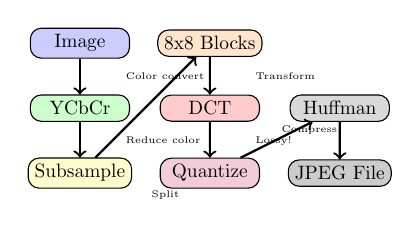
\begin{tikzpicture}[scale=0.55, every node/.style={scale=0.7}]
            % Encoding side
            \node[draw, fill=blue!20, rounded corners, minimum width=1.8cm] (img) at (0,4) {Image};
            \node[draw, fill=green!20, rounded corners, minimum width=1.8cm] (ycbcr) at (0,2.5) {YCbCr};
            \node[draw, fill=yellow!20, rounded corners, minimum width=1.8cm] (sub) at (0,1) {Subsample};
            \node[draw, fill=orange!20, rounded corners, minimum width=1.8cm] (block) at (3,4) {8x8 Blocks};
            \node[draw, fill=red!20, rounded corners, minimum width=1.8cm] (dct) at (3,2.5) {DCT};
            \node[draw, fill=purple!20, rounded corners, minimum width=1.8cm] (quant) at (3,1) {Quantize};
            \node[draw, fill=gray!30, rounded corners, minimum width=1.8cm] (huff) at (6,2.5) {Huffman};
            \node[draw, fill=black!20, rounded corners, minimum width=1.8cm] (file) at (6,1) {JPEG File};
            
            % Arrows
            \draw[->,thick] (img) -- (ycbcr);
            \draw[->,thick] (ycbcr) -- (sub);
            \draw[->,thick] (sub) -- (block);
            \draw[->,thick] (block) -- (dct);
            \draw[->,thick] (dct) -- (quant);
            \draw[->,thick] (quant) -- (huff);
            \draw[->,thick] (huff) -- (file);
            
            % Labels
            \node[right, font=\tiny] at (0.9,3.25) {Color convert};
            \node[right, font=\tiny] at (0.9,1.75) {Reduce color};
            \node[right, font=\tiny] at (1.5,0.5) {Split};
            \node[right, font=\tiny] at (3.9,3.25) {Transform};
            \node[right, font=\tiny] at (3.9,1.75) {Lossy!};
            \node[right, font=\tiny] at (4.5,2) {Compress};
        \end{tikzpicture}
    \end{center}
    
    \vspace{0.3cm}
    \textbf{Summary of each step:}
    \begin{enumerate}
        \item \textbf{YCbCr:} Separate brightness from color
        \item \textbf{Subsample:} Reduce color resolution (humans won't notice)
        \item \textbf{8x8 Blocks:} Divide and conquer
        \item \textbf{DCT:} Find patterns, concentrate energy
        \item \textbf{Quantize:} Round aggressively (this is where quality is lost)
        \item \textbf{Huffman:} Compress the numbers efficiently
    \end{enumerate}
\end{frame}

\begin{frame}{Decoding: The Reverse Journey}
    \textbf{To view a JPEG, reverse all steps:}
    
    \begin{center}
        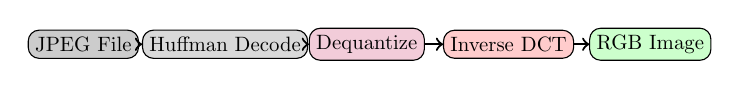
\begin{tikzpicture}[scale=0.6, every node/.style={scale=0.75}]
            \node[draw, fill=black!20, rounded corners] (file) at (0,0) {JPEG File};
            \node[draw, fill=gray!30, rounded corners] (huff) at (3,0) {Huffman Decode};
            \node[draw, fill=purple!20, rounded corners] (dequant) at (6,0) {Dequantize};
            \node[draw, fill=red!20, rounded corners] (idct) at (9,0) {Inverse DCT};
            \node[draw, fill=green!20, rounded corners] (rgb) at (12,0) {RGB Image};
            
            \draw[->,thick] (file) -- (huff);
            \draw[->,thick] (huff) -- (dequant);
            \draw[->,thick] (dequant) -- (idct);
            \draw[->,thick] (idct) -- (rgb);
        \end{tikzpicture}
    \end{center}
    
    \vspace{0.5cm}
    \begin{alertblock}{Important!}
        Decoding cannot recover the original image perfectly!
        
        The information lost during quantization is gone forever.
        
        That's why JPEG is called ``lossy'' compression.
    \end{alertblock}
\end{frame}

%==============================================================================
\section{Real-World Scenarios}
%==============================================================================

\begin{frame}{Scenario 1: Sharing Photos on WhatsApp}
    \begin{columns}
        \begin{column}{0.5\textwidth}
            \textbf{What happens when you send a photo:}
            \begin{enumerate}
                \item You take a 12 MP photo (36 MB raw)
                \item Phone saves as JPEG (3 MB)
                \item WhatsApp re-compresses to ~100 KB
                \item Friend receives smaller image
            \end{enumerate}
            
            \vspace{0.3cm}
            \textbf{Why so aggressive?}
            \begin{itemize}
                \item Faster upload/download
                \item Less mobile data used
                \item Works on slow connections
            \end{itemize}
        \end{column}
        \begin{column}{0.5\textwidth}
            \textbf{The tradeoff:}
            
            \vspace{0.3cm}
            Original: 4000 x 3000 pixels
            
            WhatsApp: 1280 x 960 pixels
            
            Quality: ~70\%
            
            \vspace{0.5cm}
            \begin{block}{Pro Tip}
                Send as ``Document'' to preserve original quality!
            \end{block}
        \end{column}
    \end{columns}
\end{frame}

\begin{frame}{Scenario 2: Website Images}
    \textbf{Why website images need careful optimization:}
    
    \vspace{0.3cm}
    \begin{columns}
        \begin{column}{0.5\textwidth}
            \textbf{Page load time matters:}
            \begin{itemize}
                \item 1 second delay = 7\% fewer sales
                \item Google ranks faster sites higher
                \item Users leave slow sites
            \end{itemize}
            
            \vspace{0.3cm}
            \textbf{Typical website image:}
            \begin{itemize}
                \item Hero image: 200-400 KB
                \item Thumbnails: 10-30 KB
                \item Icons: Use PNG/SVG instead
            \end{itemize}
        \end{column}
        \begin{column}{0.5\textwidth}
            \textbf{Best practices:}
            \begin{itemize}
                \item Quality 70-85\% for photos
                \item Resize to actual display size
                \item Use responsive images
                \item Consider WebP format
            \end{itemize}
            
            \vspace{0.3cm}
            \begin{alertblock}{Common Mistake}
                Uploading 5 MB photos that display at 500x300 pixels!
            \end{alertblock}
        \end{column}
    \end{columns}
\end{frame}

\begin{frame}{Scenario 3: Professional Photography}
    \textbf{When quality matters most:}
    
    \vspace{0.3cm}
    \begin{columns}
        \begin{column}{0.5\textwidth}
            \textbf{Workflow:}
            \begin{enumerate}
                \item Shoot in RAW format
                \item Edit in Lightroom/Photoshop
                \item Export as high-quality JPEG
                \item Keep RAW as backup
            \end{enumerate}
            
            \vspace{0.3cm}
            \textbf{Export settings:}
            \begin{itemize}
                \item Quality: 90-100\%
                \item Color space: sRGB for web
                \item Resolution: Full size
            \end{itemize}
        \end{column}
        \begin{column}{0.5\textwidth}
            \textbf{Why not just use RAW?}
            \begin{itemize}
                \item RAW files are huge (25-50 MB)
                \item Not universally supported
                \item Can't share easily
                \item JPEG is ``good enough'' for delivery
            \end{itemize}
            
            \vspace{0.3cm}
            \begin{block}{Pro Tip}
                Never edit and re-save JPEG multiple times --- quality degrades each time!
            \end{block}
        \end{column}
    \end{columns}
\end{frame}

\begin{frame}{Scenario 4: Medical Imaging}
    \begin{alertblock}{Critical Application}
        Medical images (X-rays, MRIs) often use \textbf{lossless} formats, not JPEG!
    \end{alertblock}
    
    \vspace{0.3cm}
    \textbf{Why JPEG can be dangerous for medical images:}
    \begin{itemize}
        \item Small details might indicate disease
        \item Compression artifacts could hide tumors
        \item Legal requirements for image integrity
        \item Diagnosis accuracy is critical
    \end{itemize}
    
    \vspace{0.3cm}
    \textbf{What they use instead:}
    \begin{itemize}
        \item DICOM format (medical standard)
        \item Lossless JPEG (yes, it exists!)
        \item JPEG 2000 with lossless mode
        \item PNG for some applications
    \end{itemize}
\end{frame}

\begin{frame}{Scenario 5: Social Media Memes}
    \textbf{Why do memes look so bad?}
    
    \begin{center}
        Download $\rightarrow$ Edit $\rightarrow$ Upload $\rightarrow$ Download $\rightarrow$ Edit $\rightarrow$ Upload...
    \end{center}
    
    \vspace{0.3cm}
    \begin{columns}
        \begin{column}{0.5\textwidth}
            \textbf{Generation Loss:}
            \begin{itemize}
                \item Each save loses quality
                \item Platforms re-compress
                \item Text becomes unreadable
                \item Colors get muddy
                \item Artifacts multiply
            \end{itemize}
        \end{column}
        \begin{column}{0.5\textwidth}
            \textbf{After 10+ generations:}
            \begin{itemize}
                \item Severe blocking
                \item Color banding
                \item Blurry edges
                \item ``Deep fried'' look
            \end{itemize}
            
            \vspace{0.3cm}
            \textit{This is actually used as an aesthetic in ``deep fried memes''!}
        \end{column}
    \end{columns}
\end{frame}

%==============================================================================
\section{JPEG vs Other Formats}
%==============================================================================

\begin{frame}{When to Use JPEG}
    \begin{columns}
        \begin{column}{0.5\textwidth}
            \textbf{JPEG is GREAT for:}
            \begin{itemize}
                \item Photographs
                \item Natural images
                \item Complex scenes
                \item Gradients and shadows
                \item Web photos
                \item Social media
            \end{itemize}
        \end{column}
        \begin{column}{0.5\textwidth}
            \textbf{JPEG is BAD for:}
            \begin{itemize}
                \item Text and logos
                \item Screenshots
                \item Line art
                \item Images with transparency
                \item Graphics with sharp edges
                \item Images needing editing
            \end{itemize}
        \end{column}
    \end{columns}
    
    \vspace{0.5cm}
    \begin{block}{Simple Rule}
        \textbf{Photo?} $\rightarrow$ JPEG \hspace{1cm} \textbf{Graphics/Text?} $\rightarrow$ PNG
    \end{block}
\end{frame}

\begin{frame}{Format Comparison}
    \begin{center}
        \begin{tabular}{l|c|c|c|c}
            \toprule
            \textbf{Feature} & \textbf{JPEG} & \textbf{PNG} & \textbf{WebP} & \textbf{HEIC} \\
            \midrule
            Compression & Lossy & Lossless & Both & Both \\
            Transparency & No & Yes & Yes & Yes \\
            Animation & No & No & Yes & Yes \\
            File Size & Small & Large & Smaller & Smallest \\
            Quality & Good & Perfect & Better & Best \\
            Support & Universal & Universal & Good & Apple \\
            \bottomrule
        \end{tabular}
    \end{center}
    
    \vspace{0.5cm}
    \textbf{The future:}
    \begin{itemize}
        \item WebP is replacing JPEG on the web
        \item HEIC is default on iPhones
        \item AVIF is the newest contender
        \item But JPEG will be around for decades!
    \end{itemize}
\end{frame}

%==============================================================================
\section{Summary}
%==============================================================================

\begin{frame}{Key Takeaways}
    \begin{enumerate}
        \item \textbf{JPEG exploits human vision} --- we don't see all details equally
        
        \item \textbf{Six-step pipeline:} Color convert $\rightarrow$ Subsample $\rightarrow$ Block $\rightarrow$ DCT $\rightarrow$ Quantize $\rightarrow$ Encode
        
        \item \textbf{Quantization is the lossy step} --- this is where quality vs size tradeoff happens
        
        \item \textbf{Quality 70-85\%} is usually the sweet spot
        
        \item \textbf{Don't re-save JPEGs} --- quality degrades each time
        
        \item \textbf{Use JPEG for photos}, PNG for graphics
    \end{enumerate}
\end{frame}

\begin{frame}{Quick Reference}
    \begin{block}{JPEG Quality Guide}
        \begin{itemize}
            \item \textbf{100\%:} Maximum quality, large files (archival)
            \item \textbf{90-95\%:} Excellent quality, professional use
            \item \textbf{75-85\%:} Good quality, web/social media
            \item \textbf{50-70\%:} Acceptable, thumbnails
            \item \textbf{Below 50\%:} Visible artifacts, avoid
        \end{itemize}
    \end{block}
    
    \vspace{0.3cm}
    \begin{block}{File Size Estimates (12 MP photo)}
        \begin{itemize}
            \item RAW: 25-50 MB
            \item JPEG 100\%: 8-12 MB
            \item JPEG 80\%: 2-4 MB
            \item JPEG 50\%: 500 KB - 1 MB
        \end{itemize}
    \end{block}
\end{frame}

\begin{frame}
    \begin{center}
        \Huge{\textbf{Thank You!}}
        
        \vspace{1cm}
        \Large{Questions?}
        
        \vspace{1.5cm}
        \normalsize
        \textit{``JPEG: Making the internet possible since 1992''}
        
        \vspace{0.5cm}
        \small{Next class: Video compression and how YouTube works!}
    \end{center}
\end{frame}

\end{document}
